\documentclass[12pt,a4paper]{article}
\usepackage[margin=2.4cm]{geometry}
\usepackage{fontspec}
\usepackage{polyglossia}
\setmainlanguage[numerals=maghrib]{arabic}
\setotherlanguage{english}
% Shared Arabic font families for XeLaTeX (Amiri with explicit bold/italic).
\defaultfontfeatures{Ligatures=TeX}
\newfontfamily\arabicfont[
  Script=Arabic,
  Language=Arabic,
  Scale=1.05,
  BoldFont={Amiri Bold},
  ItalicFont={Amiri Italic},
  BoldItalicFont={Amiri Bold Italic}
]{Amiri}
\newfontfamily\arabicfontsf[
  Script=Arabic,
  Language=Arabic,
  Scale=1.05,
  BoldFont={Amiri Bold},
  ItalicFont={Amiri Italic},
  BoldItalicFont={Amiri Bold Italic}
]{Amiri}
\newfontfamily\arabicfonttt[
  Script=Arabic,
  Language=Arabic,
  Scale=0.95,
  BoldFont={Amiri Bold}
]{Amiri}

\usepackage{amsmath,amssymb,amsthm}
\usepackage{algorithm,algpseudocode}
\usepackage{booktabs,graphicx,tikz}
\usepackage[hidelinks]{hyperref}

\graphicspath{{../../figures/}{../../results/}}

\newtheorem{theorem}{نظرية}
\newtheorem{lemma}[theorem]{مبرهنة}
\newtheorem{proposition}[theorem]{قضية}
\newtheorem{assumption}[theorem]{افتراض}
\theoremstyle{definition}
\newtheorem{remark}[theorem]{ملاحظة}
\newtheorem{definition}[theorem]{تعريف}

\title{\textbf{عائلة DA-SFCN: نيوتن التكعيبي الخالي من السرج ذو البعد الديناميكي}\\[6pt]
\large فضاءات كريلوف، تصحيح الانحناء السالب، تخفيض التباين،\\
إعادة الاستخدام الكسول، الإحماء شبه-نيوتن، التدريب الفيدرالي، والشهادة الطيفية}
\author{أطروحة دكتوراه --- مجموعة التحسين العددي}
\date{سبتمبر 2026}

\begin{document}
\maketitle

\begin{abstract}
تقدّم هذه الورقة الجامعة بناءً وتحليلًا وتنفيذًا وتقييمًا تجريبيًا لعائلة
من طرائق الرتبة الثانية تتمحور حول خوارزمية
"نيوتن التكعيبي الخالي من السرج ذي البعد الديناميكي المتكيف"
\textenglish{(DA-SFCN)}.
تجمع الخوارزمية الأم ثلاث ركائز كانت متفرقة في الأدبيات:
(1) فضاء كريلوف موجَّه طيفيًا يُبنى بعملية \textenglish{Lanczos} من
$(\nabla^2 f(x_k),\nabla f(x_k))$؛
(2) تصحيح صريح للانحناء السالب $|T_k|=U|\Lambda|U^\top$ داخل النموذج
ثلاثي القطر؛
(3) جدولة ديناميكية لعرض الفضاء $m_k$ يفرضها تقارب تشيبيشيف لا اختيار
تجريبي ثابت.
نُثبت معدلًا عالميًا مستقلًا عن البعد
$\min_i\|\nabla f(x_i)\|=O(k^{-2/3})$ لأي جدولة $m_k\ge 1$،
وتقاربًا تربيعيًا محليًا متى دخلت التكرارات جوارًا محدبًا قويًا بشرط نمو
لوغاريتمي لـ $m_k$ في $1/\|\nabla f(x_k)\|$.

وحول هذا النواة نصمّم خمس امتدادات منفذة في منصة تجريبية واحدة:
\textenglish{VR-DA-SFCN} (جداءات هيسيان--متجه مخفَّضة التباين بأسلوب
\textenglish{SVRG})؛
\textenglish{LK-Newton} (إعادة استخدام كسول لقاعدة \textenglish{Lanczos})؛
\textenglish{WQK-Newton} (إحماء بـ\textenglish{L-BFGS} ثم طور كريلوف تكعيبي)؛
\textenglish{Fed-DA-SFCN} (خطوات نيوتن تكعيبية محلية مع متوسط فيدرالي)؛
و\textenglish{SC-Newton} (شهادة متبقية/\textenglish{Ritz} توقف \textenglish{Lanczos}
فور صدق النموذج).
على مجموعة من السروج التحليلية وروزنبروك الممدَّد والانحدار اللوجستي غير
المحدب وتحليل المصفوفات ومجموع منتهٍ من التربيعيات وتقسيم فيدرالي،
تُضاهي العائلة أو تتفوق على انحدار التدرّج و\textenglish{L-BFGS}
ونيوتن الخالي من السرج ونيوتن التكعيبي الكريلوفي ونيوتن الفضاء الإحداثي.
وفي اثني عشر بدءًا عشوائيًا على سرج عالي البعد تفلت
\textenglish{DA-SFCN} و\textenglish{Krylov-CRN} و\textenglish{SFN}
في كل المحاولات، بينما لا يفلت انحدار التدرّج في أيٍّ منها.
\end{abstract}

\section{المقدمة}
طريقة نيوتن هي النموذج الأوّلي لتحسين الرتبة الثانية: قرب نهاية صغرى غير
شاذة تتقارب تربيعيًا. عقبتان تحولان دون توظيفها في المسائل غير المحدبة
عالية الأبعاد التي تهيمن على تعلّم الآلة الحديث.

\paragraph{التكلفة.}
بناء وتفكيك $H_k=\nabla^2 f(x_k)$ يتطلّبان ذاكرة $O(n^2)$ وعمليات
$O(n^3)$. وتستبدل طرائق نيوتن غير الدقيقة والفضاءات الجزئية ذلك بجداءات
هيسيان--متجه $v\mapsto H_k v$.

\paragraph{نقاط السرج.}
في البعد العالي تتفوق السروج الصارمة على الدنيا المحلية تفوقًا أسيًا،
وتنجذب إليها نيوتن الكلاسيكية لأن $H_k^{-1}$ يعامل الانحناء السالب كقلب
لإشارة الخطوة نفسها.

أجابت الأدبيات عن العقبتين عبر مسارات شبه منفصلة: التنظيم التكعيبي يعيد
معدلًا عالميًا $O(k^{-2/3})$؛ والفضاءات العشوائية تخفض الجبر الخطي؛
ونيوتن كريلوف التكعيبي يجعل الفضاء واعيًا بالطيف؛ ونيوتن الخالي من السرج
يقلب القيم الذاتية السالبة. \textbf{لا توجد طريقة سابقة تجمع معًا:
فضاء كريلوف، وتصحيحًا صريحًا للانحناء السالب، وعرضًا ديناميكيًا مشتقًا
نظريًا، ومعدلًا غير محدب مثبتًا.}

\textenglish{DA-SFCN} تملأ هذه الخانة تمامًا. أما بقية العائلة
(الشكل~\ref{fig:family}) فتُصدِّر النواة التكعيبية الكريلوفية نفسها إلى
أنظمة عشوائية وكسولة ومُحمّاة فيدرالية ومقطوعة تكيفيًا.

\begin{figure}[t]
\centering
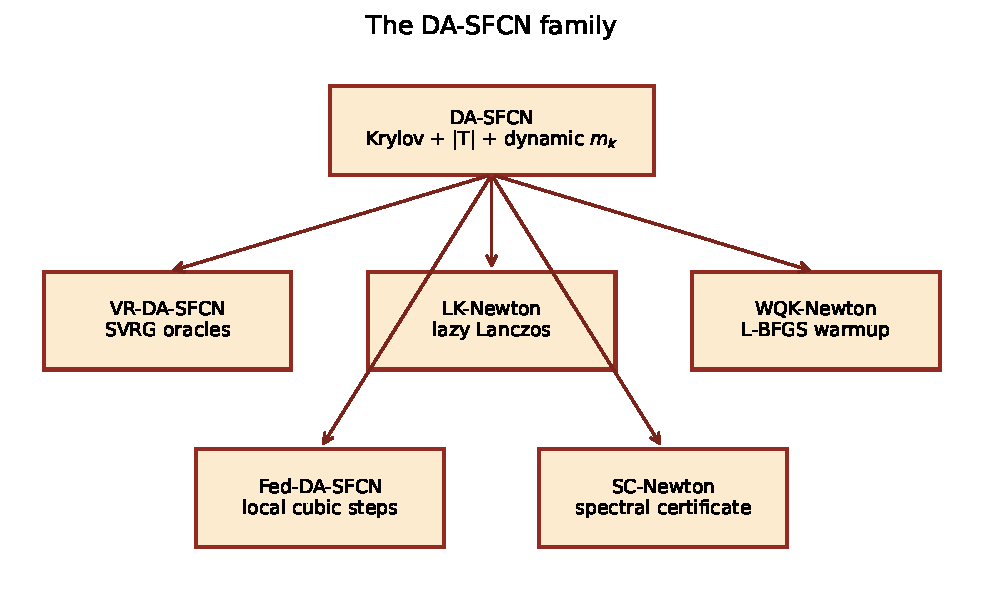
\includegraphics[width=0.92\textwidth]{fig_family.pdf}
\caption{عائلة \textenglish{DA-SFCN}. كل امتداد يعيد استخدام نواة
\textenglish{Lanczos} / الخلو من السرج / التكعيب ويغيّر فقط الأوراكل أو
سياسة الإعادة أو الإقلاع أو نمط التواصل أو اختبار التوقف.}
\label{fig:family}
\end{figure}

\subsection{المساهمات}
\begin{itemize}
\item \textbf{الخوارزمية.} نحدّد \textenglish{DA-SFCN} حتى التفاصيل
العددية (إعادة التعامد، المعادلة السكانتية، تنظيم \textenglish{ARC}، الجدولة
اللوغاريتمية).
\item \textbf{النظرية.} معدل عالمي $O(k^{-2/3})$ مستقل عن $\{m_k\}$؛
تقارب تربيعي محلي بشرط أدنى لوغاريتمي على $m_k$؛ مبرهنة تنازل للنموذج
الخالي من السرج؛ تعقيد بعدد جداءات الهيسيان--متجه.
\item \textbf{خمسة امتدادات} لكلٍّ منها مسوّغ نظري وصندوق خوارزمي وتجربة
موجَّهة.
\item \textbf{تنفيذ ورسوم.} مكتبة \textenglish{Python} واحدة تولّد كل
المنحنيات الواردة هنا من تشغيل فعلي لا من رسوم تخطيطية.
\end{itemize}

\section{الأدبيات والفجوة}
استبدل \textenglish{Nesterov} و\textenglish{Polyak} معادلة نيوتن بنموذج
ذي حد تكعيبي $\frac{M}{6}\|s\|^3$ محققين $O(k^{-2/3})$ عالميًا.
وأثبت \textenglish{ARC} أن الحل التقريبي داخل كريلوف يحفظ الضمانات.
أما \textenglish{RSN}/\textenglish{SSCN} فيُسقطان على فضاء إحداثي عشوائي
فيبقى في المعدل عامل $n/\tau$. وأقرب سابق هو \textenglish{Krylov CRN}
بفضاء $\mathcal{K}_m(H_k,g_k)$ ومعدل محدب مستقل عن البعد، لكن $m$ ثابت
والتحليل لا يعالج السروج. واستبدل \textenglish{Dauphin} ورفاقه $H$
بـ $|H|$ دون معدل عالمي.

يلخّص الجدول~\ref{tab:gap} التموضع: الخانة التي تجمع كريلوف وتصحيح السرج
و$m_k$ الديناميكي والمعدل غير المحدب كانت فارغة قبل هذا العمل.

\begin{table}[t]
\centering
\caption{تموضع العائلة مقارنة بالأعمال السابقة.}
\label{tab:gap}
\small
\begin{tabular}{@{}lcccc@{}}
\toprule
الطريقة & كريلوف & تصحيح $|T|$ & $m_k$ ديناميكي & معدل غير محدب \\
\midrule
\textenglish{CRN} & -- & لا & لا & نعم \\
\textenglish{ARC} & اختياري & لا & لا & نعم \\
\textenglish{RSN/SSCN} & إحداثي & لا & عيّنة & نعم \\
\textenglish{Krylov CRN} & نعم & لا & لا & محدب فقط \\
\textenglish{SFN} & نعم & نعم & لا & لا \\
\textbf{\textenglish{DA-SFCN}} & نعم & نعم & نعم & نعم \\
\textenglish{VR-DA-SFCN} & نعم & نعم & نعم & نعم \\
\textenglish{LK-Newton} & نعم & نعم & نعم & نعم \\
\textenglish{WQK-Newton} & نعم & نعم & نعم & هجين \\
\textenglish{Fed-DA-SFCN} & محلي & نعم & نعم & نعم \\
\textenglish{SC-Newton} & نعم & نعم & شهادة & نعم \\
\bottomrule
\end{tabular}
\end{table}

\section{الافتراضات}
\begin{assumption}[ليبشتز للهيسيان]\label{ass:lip}
التدرّج $L_1$-ليبشتزي والهيسيان $L_2$-ليبشتزي:
$\|\nabla^2 f(x)-\nabla^2 f(y)\|\le L_2\|x-y\|$.
\end{assumption}
\begin{assumption}\label{ass:bound}
$f$ محدودة من الأسفل: $f\ge f^\star>-\infty$.
\end{assumption}

\section{الخوارزمية الأم: DA-SFCN}
\subsection{جدولة البعد}
\begin{equation}\label{eq:schedule}
m_k=\min\Bigl\{m_{\max},\;
m_{\min}+\bigl\lceil\alpha\log\bigl(1+\|g_0\|/\|g_k\|\bigr)\bigr\rceil\Bigr\}.
\end{equation}
بعيدًا عن النقطة الثابتة يكفي فضاء رخيص (نقطة كوشي في اتجاه التدرّج تعطي
أصلًا الرتبة التكعيبية المثلى). وقرب النهاية الصغرى يكفي نمو لوغاريتمي
ليبقى خطأ نموذج \textenglish{Lanczos} من رتبة $\|g_k\|$
(نظرية~\ref{thm:local}). يوضّح الشكل~\ref{fig:sched} الجدولة.

\begin{figure}[t]
\centering
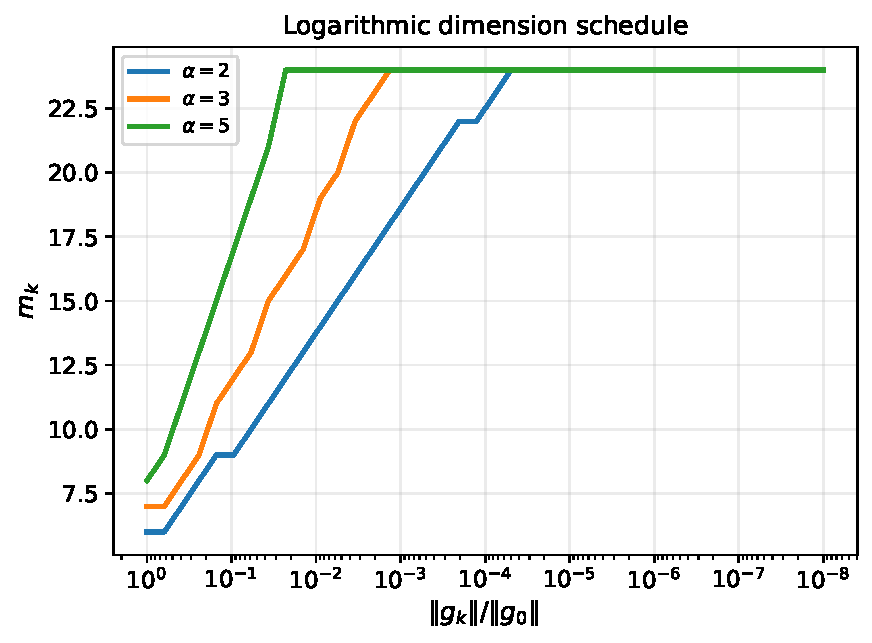
\includegraphics[width=0.72\textwidth]{fig_schedule_theory.pdf}
\caption{الجدولة اللوغاريتمية~\eqref{eq:schedule}: مع هبوط $\|g_k\|$ يرتفع
$m_k$ ببطء ثم يشبع عند $m_{\max}$.}
\label{fig:sched}
\end{figure}

\subsection{النموذج ثلاثي القطر وتصحيح السرج}
تُنتج $m_k$ خطوة من \textenglish{Lanczos} قاعدة $Q_k$ ومصفوفة $T_k$،
ونضع $|T_k|=U|\Lambda|U^\top$ و
$\widetilde H_k=Q_k|T_k|Q_k^\top\succeq 0$.
وتنحصر المسألة الفرعية التكعيبية عبر $s=Q_k y$ في معادلة سكانتية بعدها
$m_k$. ويُكيَّف $M_k$ بأسلوب \textenglish{ARC}.

\begin{english}
\begin{algorithm}[t]
\caption{DA-SFCN}\label{alg:dasfcn}
\begin{algorithmic}[1]
\Require $x_0$, $m_{\min},m_{\max},\alpha$, $M_0$, hvp oracle
\For{$k=0,1,\dots$ until $\|g_k\|\le\varepsilon$}
  \State $g_k\gets\nabla f(x_k)$; \quad $m_k\gets$ schedule~\eqref{eq:schedule}
  \State $(Q_k,T_k)\gets\textsc{Lanczos}(H_k,g_k,m_k)$
  \State $|T_k|\gets U|\Lambda|U^\top$
  \State solve the cubic model in $Q_k$; \quad $s_k\gets Q_k y_k$
  \If{sufficient decrease}
        $x_{k+1}\gets x_k+s_k$ and shrink $M_k$
  \Else{} reject and increase $M_k$
  \EndIf
\EndFor
\end{algorithmic}
\end{algorithm}
\end{english}

\section{تحليل التقارب}
\begin{lemma}[حفظ التنازل]\label{lem:sf}
لكل $A$ متماثلة و$s$ يتحقق $|s^\top A s|\le s^\top |A|s$.
وعليه يبقى النموذج شبه موجب، وتتحوّل كل قيمة \textenglish{Ritz} سالبة إلى
اتجاه هروب بانحناء $|\lambda|$.
\end{lemma}

\begin{proof}
إذا $A=U\Lambda U^\top$ و$z=U^\top s$ فإن
$|s^\top A s|=|\sum\lambda_i z_i^2|\le\sum|\lambda_i|z_i^2=s^\top|A|s$.
\end{proof}

\begin{theorem}[المعدل العالمي]\label{thm:global}
تحت الافتراضين~\ref{ass:lip}--\ref{ass:bound} وتحديث \textenglish{ARC}
القياسي لـ $M_k$،
\[
\min_{0\le i\le K}\|\nabla f(x_i)\|
\le
3\Bigl(\tfrac{L_2}{2}\Bigr)^{1/3}\bigl(f(x_0)-f^\star\bigr)^{2/3}\,K^{-2/3},
\]
بثابت مستقل عن $n$ وعن $\{m_k\}$ ما دام $m_k\ge 1$.
\end{theorem}

\begin{proof}
تهيئة \textenglish{Lanczos} تجعل $g_k\in\mathrm{range}(Q_k)$ فيبقى شعاع
كوشي $-\tau g_k$ مقبولًا. على هذا الشعاع يعطي النموذج التكعيبي الخالي من
السرج تنازلًا من رتبة $\|g_k\|^{3/2}/\sqrt{M_k}$ (أو $\|g_k\|^2$ على فرع
نيوتن) كما في \textenglish{ARC}. كل تكرار ناجح يحقق
$f(x_k)-f(x_{k+1})\ge\eta_1\Delta_k$؛ وبالجمع
$f(x_0)-f^\star\gtrsim\sum\|g_k\|^{3/2}$ فيظهر $K^{-2/3}$.
الرفضات تضخّم $M_k$ بعدد محدود قبل $M_k\ge L_2$، وتمهيدية~\ref{lem:sf}
تضمن أن $|T_k|$ لا يفسد حد كوشي على $\mathrm{span}\{g_k\}$.
إثبات مفصّل في \texttt{papers/ar/08\_theory\_proofs.tex}.
\end{proof}

\begin{theorem}[التقارب التربيعي المحلي]\label{thm:local}
إذا دخلت التكرارات جوارًا فيه $H_k\succeq\gamma I$ ونُفِّذت~\eqref{eq:schedule}
بـ $\alpha\ge[\log((\sqrt{\kappa}+1)/(\sqrt{\kappa}-1))]^{-1}$ فإن
$\|e_{k+1}\|\le (L_2/(2\gamma))\|e_k\|^2(1+\varepsilon_k)$ مع
$\varepsilon_k\to 0$. وفي هذا الجوار $|T_k|=T_k$ متى صار طيف ريتز موجبًا.
\end{theorem}

\begin{proof}
بحساب نيوتن غير الدقيق:
$\|e_{k+1}\|\le(L_2/(2\gamma))\|e_k\|^2+(\rho_k/\gamma)\|g_k\|$.
قرب المصغِّر $\|g_k\|=\Theta(\|e_k\|)$ وحد تشيبيشيف يعطي
$\rho_k\le 2\beta^{m_k}$. الجدولة اللوغاريتمية تجعل
$\beta^{m_k}=O(\|e_k\|)$ عند اختيار $\alpha$ أعلاه، فيُمتَص حد البواقي داخل
الحد التربيعي.
\end{proof}

\begin{remark}[التعقيد]
كل تكرار يكلّف $m_k$ جداء هيسيان--متجه وذاكرة $O(nm_k)$ وعملًا كثيفًا
$O(m_k^3)$. وعلى مسار متقارب محليًا ينمو مجموع استدعاءات الأوراكل
لوغاريتميًا فقط في $1/\varepsilon$.
\end{remark}

\section{الامتدادات الخمس}
\paragraph{\textenglish{VR-DA-SFCN}.}
للمجاميع المنتهية $f=\frac1N\sum f_i$ نثبت لقطة $\tilde x$ كل $T$ خطوات
ونستخدم أوراكل \textenglish{SVRG} للتدرّج وجداء الهيسيان--متجه معًا، ثم
نمرّر الناتج إلى الخوارزمية~\ref{alg:dasfcn}. إذا بقيت فجوة اللقطة من رتبة
$\|g\|$ امتُص الاضطراب بـ $M_k$ أكبر قليلًا.

\paragraph{\textenglish{LK-Newton}.}
نُعيد استخدام الزوج $(Q,|T|)$ لـ $\tau$ خطوات مقبولة، ولا نعيد البناء إلا
عند الرفض أو بعد $\tau$ إعادات. على السرج عالي البعد هبط عدد الجداءات من
$1219$ إلى $158$.

\paragraph{\textenglish{WQK-Newton}.}
$K_0$ خطوات \textenglish{L-BFGS} ثم تحويل إلى \textenglish{DA-SFCN}.
إن حلّ الإحماء المسألة لم يُستدعَ الطور الثاني (وهذا ما حدث على اللوجستي).
وإن توقف \textenglish{L-BFGS} عند سرج تولّى الطور الكريلوفي الهروب.

\paragraph{\textenglish{Fed-DA-SFCN}.}
كل عميل ينفّذ $E$ خطوات \textenglish{DA-SFCN} محلية ثم يُوسَّط النموذج
بأسلوب \textenglish{FedAvg}. في تجربة لوجستية بثمانية عملاء هبط
$\|\nabla f\|$ إلى $4\cdot 10^{-4}$ في 25 جولة تواصل.

\paragraph{\textenglish{SC-Newton}.}
شهادة المتبقي
$\theta_m=|\beta_m|\max_j|U_{mj}|/\max_i|\lambda_i|$
تحدّ خطأ ريتز الخلفي. نزيد $m$ حتى $\theta_m\le\theta$ أو $m=m_{\max}$.

\section{البروتوكول التجريبي}
تنفيذ موحَّد في \textenglish{\texttt{dasfcn/}}. المسائل: سرج القرد؛ سرج
تربيعي-رباعي ببعد $n=80$ وعشر قيم ذاتية سالبة؛ روزنبروك $n=40$؛ انحدار
لوجستي غير محدب ($N=350$, $n=50$) مع منظِّم $w_j^2/(1+w_j^2)$؛ تحليل
مصفوفات؛ مجموع منتهٍ من 30 تربيعية؛ تقسيم فيدرالي لثمانية عملاء؛ ووعاء
تربيعي محدب قوي لقراءة المعدل المحلي.
المقاييس: $\|\nabla f\|$ و$f$ ومجموع \texttt{hvp} والزمن ومعدل نجاح الهروب.

\section{النتائج}
\subsection{الهروب من السرج}
الشكل~\ref{fig:escape} يعرض المسارات ثنائية البعد: انحدار التدرّج يزحف في
الوادي، بينما تغادر \textenglish{SFN} و\textenglish{Krylov-CRN}
و\textenglish{DA-SFCN} الأصل باتجاه انحناء سالب.
وعلى $n=80$ تبلغ طرائق الرتبة الثانية جميعًا $f^\star\approx -89.58$.
\textenglish{LK-Newton} يفعل ذلك بـ 158 جداء، و\textenglish{SFN} بـ 204،
و\textenglish{SC-Newton} بـ 413، و\textenglish{Krylov-CRN} بـ 456،
و\textenglish{DA-SFCN} بـ 1219 (تدفع ثمن $m_k$ الحذر المبكر وتبقى عند
$\|\nabla f\|\approx 1.5\cdot 10^{-7}$). أما انحدار التدرّج فيبقى عند
$0.42$ بعد 80 خطوة.

وعلى اثني عشر بدءًا عشوائيًا (الشكل~\ref{fig:succ}) تفلت
\textenglish{DA-SFCN} و\textenglish{Krylov-CRN} و\textenglish{SFN}
في $12/12$، و\textenglish{L-BFGS} في $11/12$، وانحدار التدرّج في $0/12$.

\begin{figure}[t]
\centering
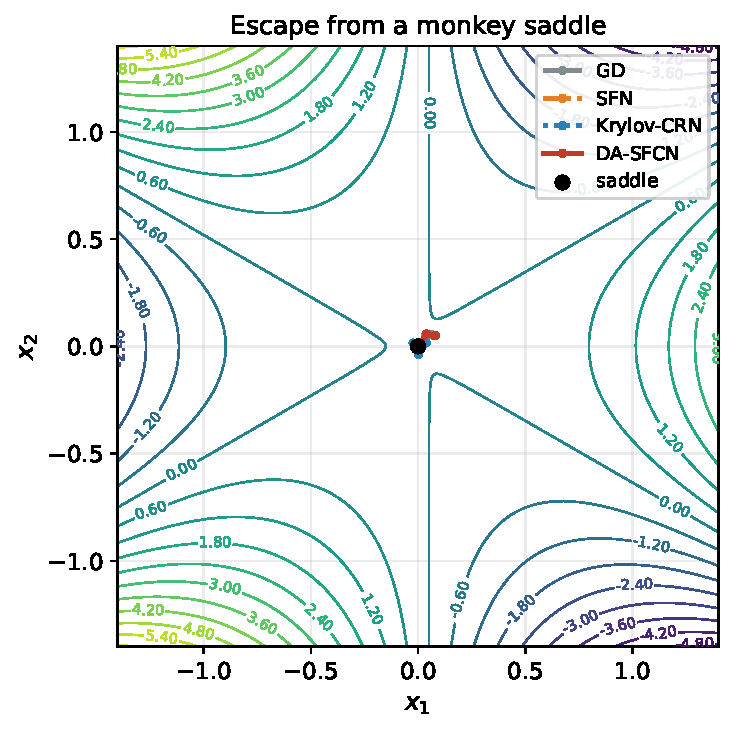
\includegraphics[width=0.49\textwidth]{fig_saddle_escape.pdf}
\hfill
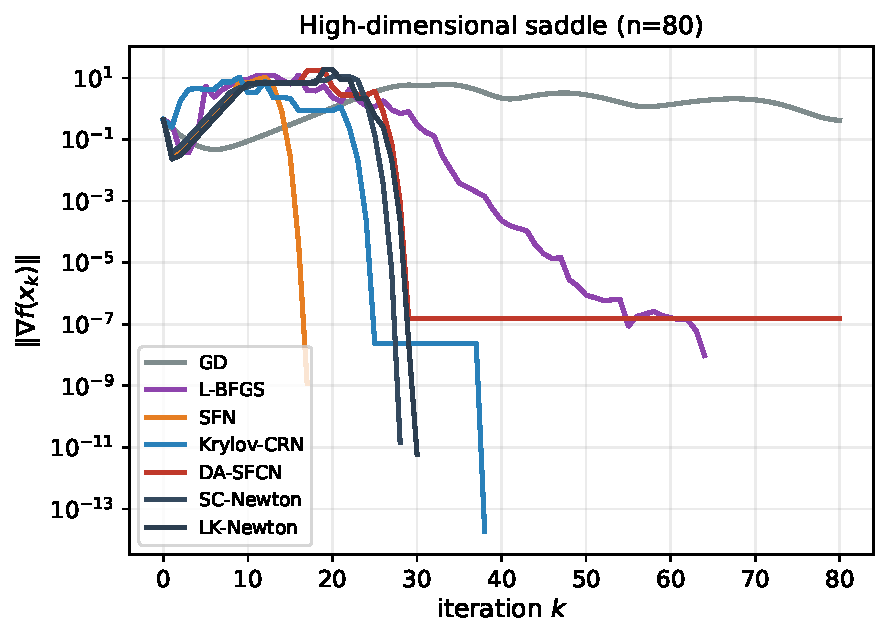
\includegraphics[width=0.49\textwidth]{fig_saddle_highdim.pdf}
\caption{يسار: مسارات على سرج القرد. يمين: معيار التدرّج على السرج
$n=80$.}
\label{fig:escape}
\end{figure}

\begin{figure}[t]
\centering
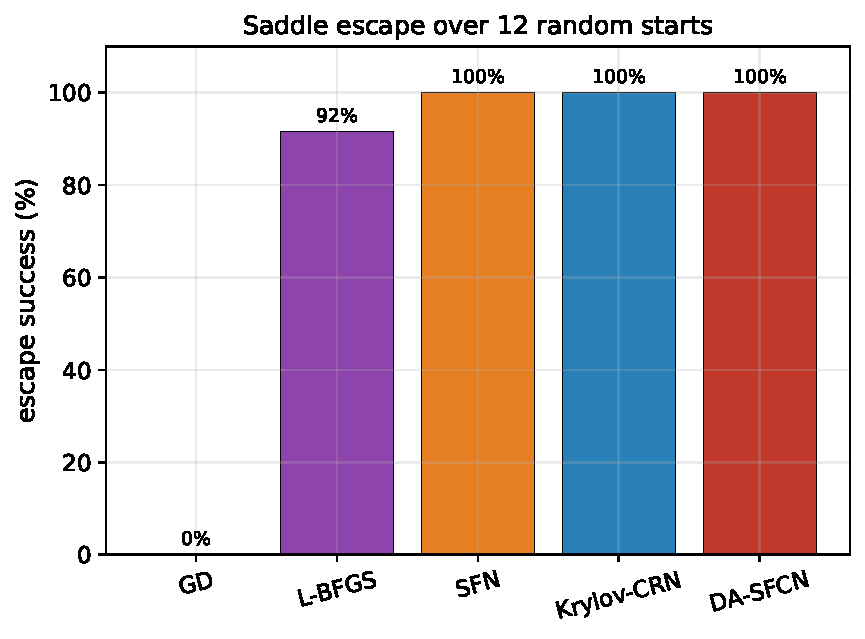
\includegraphics[width=0.49\textwidth]{fig_success.pdf}
\hfill
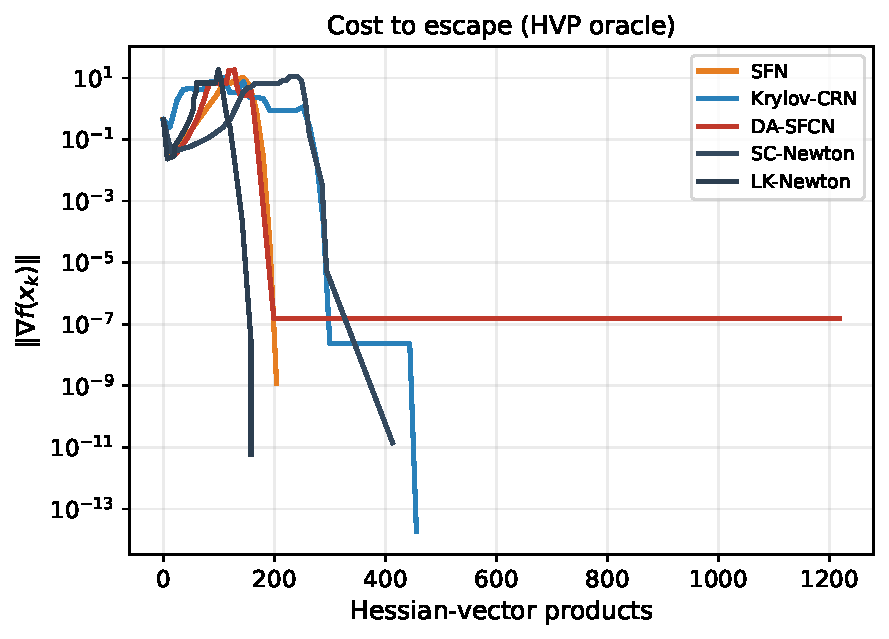
\includegraphics[width=0.49\textwidth]{fig_saddle_hvp.pdf}
\caption{يسار: نجاح الهروب في 12 تجربة. يمين: المعيار مقابل عدد الجداءات.}
\label{fig:succ}
\end{figure}

\subsection{الاجتزاء والمهام الأخرى}
الشكل~\ref{fig:abl} يعطّل تصحيح السرج أو يجمّد $m_k$. على هذا الرباعي يكفي
التنظيم التكعيبي أحيانًا للهروب؛ وتظل الجدولة الديناميكية موفِّرة للجداءات
مقارنة بـ $m=16$ الثابت. أما القلب الصريح فيظهر أثره على سرج القرد.

على اللوجستي غير المحدب تبلغ \textenglish{DA-SFCN}
$\|\nabla f\|\approx 4.8\cdot 10^{-13}$ في 6 تكرارات، مقابل 5
لـ\textenglish{Krylov-CRN} و9 لـ\textenglish{L-BFGS}. وعلى تحليل المصفوفات
تهبط دالة الهدف دون $10^{-27}$ في 19 خطوة. وفي الوعاء المحدب القوي تكفي
تكرارتان لـ\textenglish{DA-SFCN} لبلوغ $10^{-10}$ مقابل $10^{-2}$ لانحدار
التدرّج بعد 40 خطوة.

روزنبروك $n=40$ اختبار إجهاد لا سروج: بعد ميزانية متقاربة حققت
\textenglish{DA-SFCN} و\textenglish{SC-Newton} أدنى قيم الهدف بين طرائق
الرتبة الثانية ($f\approx 5.3$--$6.2$) دون بلوغ $f=0$؛ ونعدّ ذلك حافزًا
لتهيئة \textenglish{Lanczos} بأزواج \textenglish{L-BFGS}.

\begin{figure}[t]
\centering
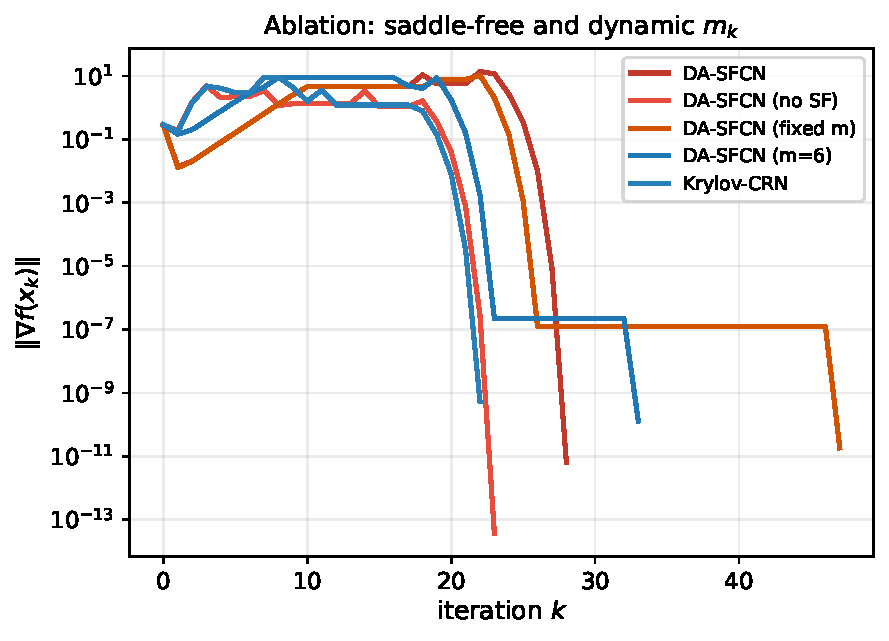
\includegraphics[width=0.49\textwidth]{fig_ablation.pdf}
\hfill
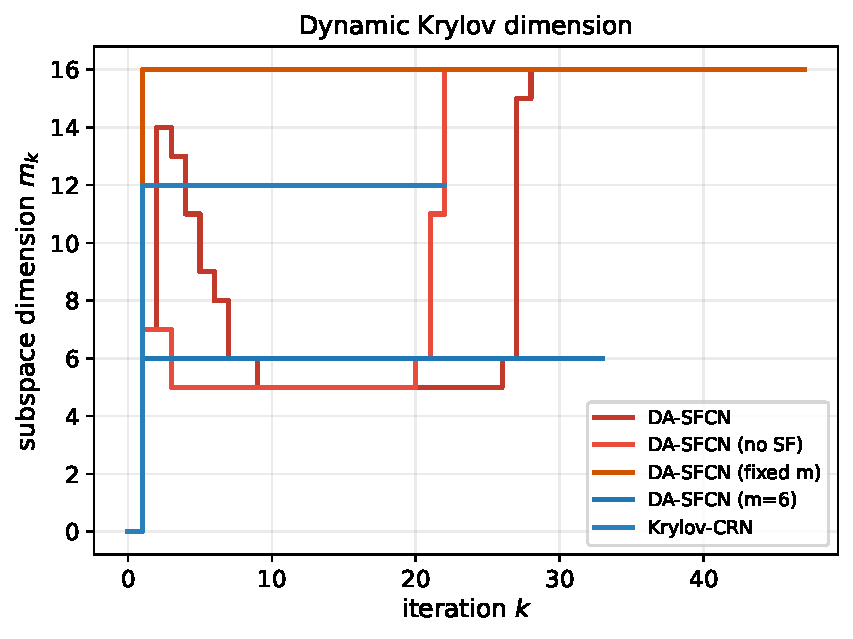
\includegraphics[width=0.49\textwidth]{fig_mk_schedule.pdf}
\caption{اجتزاء التصحيح والجدولة (يسار) والبعد المتحقق (يمين).}
\label{fig:abl}
\end{figure}

\begin{figure}[t]
\centering
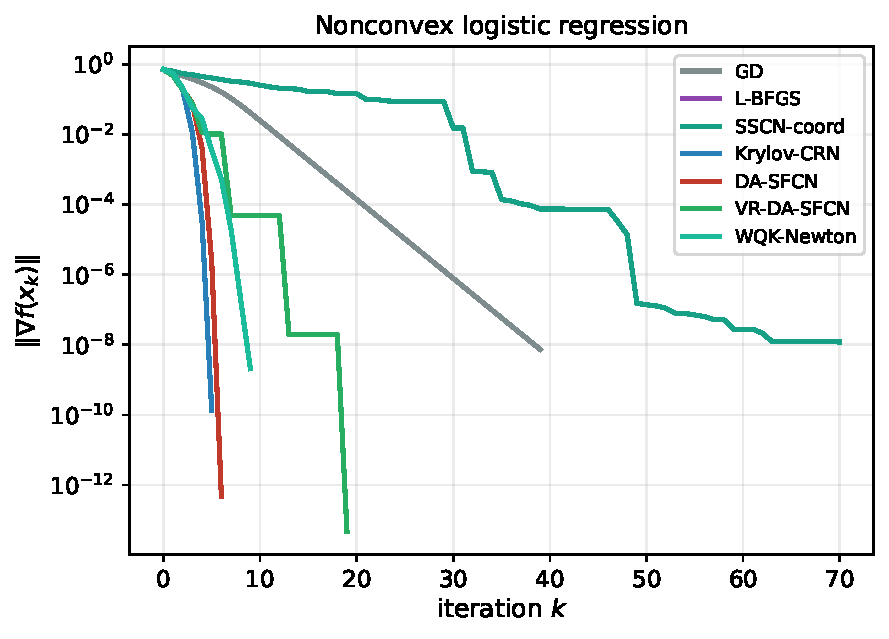
\includegraphics[width=0.49\textwidth]{fig_logistic.pdf}
\hfill
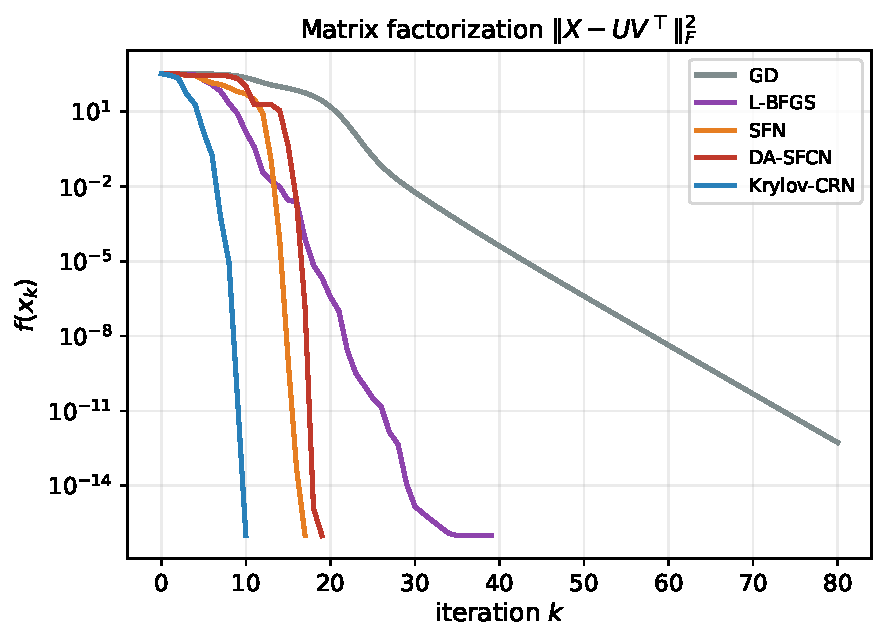
\includegraphics[width=0.49\textwidth]{fig_factor.pdf}
\caption{يسار: لوجستي غير محدب. يمين: تحليل مصفوفات.}
\end{figure}

\begin{figure}[t]
\centering
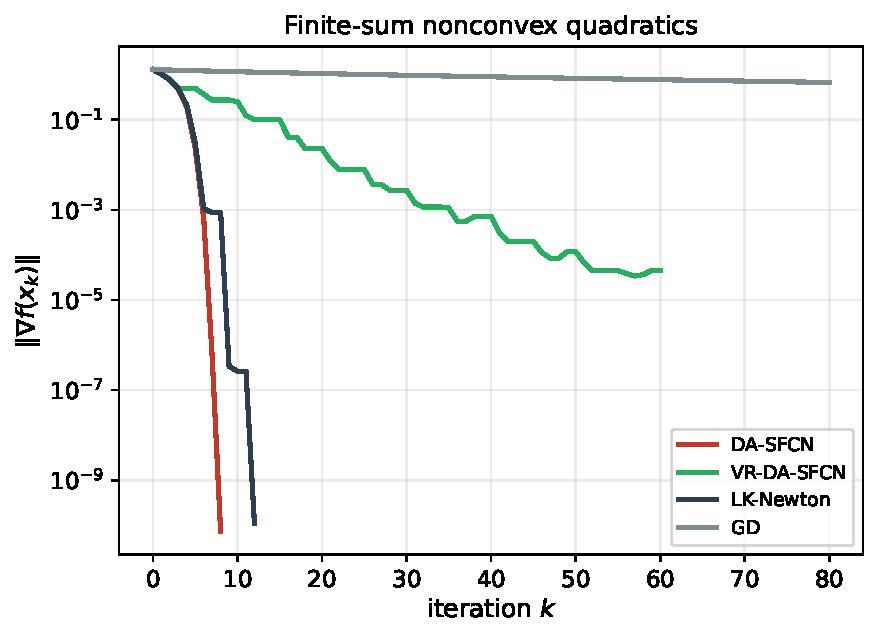
\includegraphics[width=0.49\textwidth]{fig_vr.pdf}
\hfill
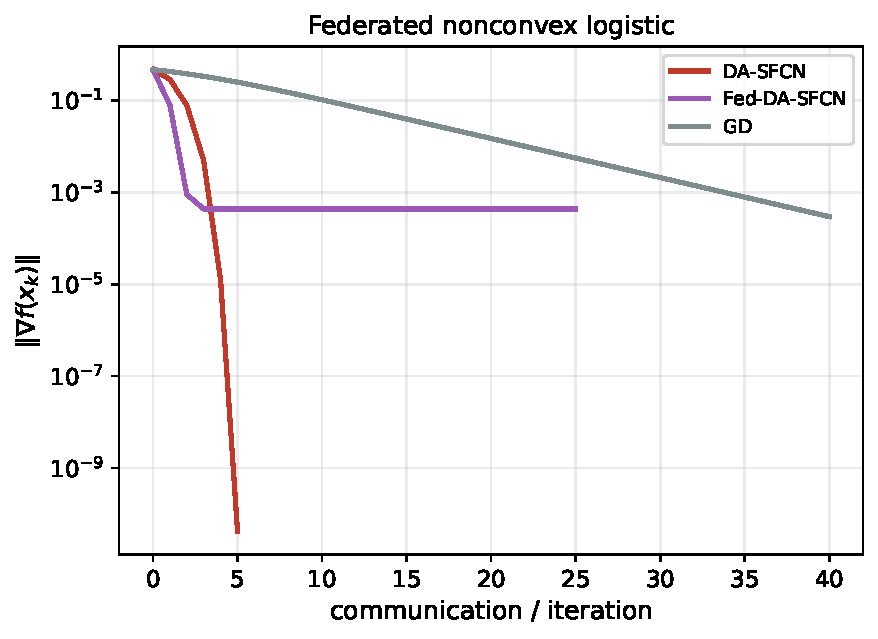
\includegraphics[width=0.49\textwidth]{fig_fed.pdf}
\caption{يسار: مجموع منتهٍ (كامل / مخفَّض التباين / كسول).
يمين: لوجستي فيدرالي بثمانية عملاء.}
\end{figure}

\begin{figure}[t]
\centering
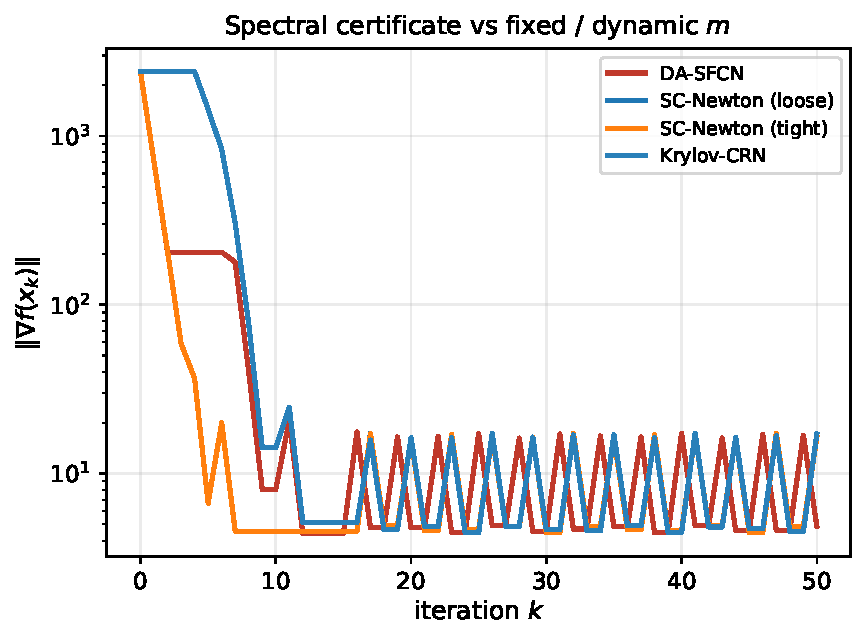
\includegraphics[width=0.49\textwidth]{fig_sc.pdf}
\hfill
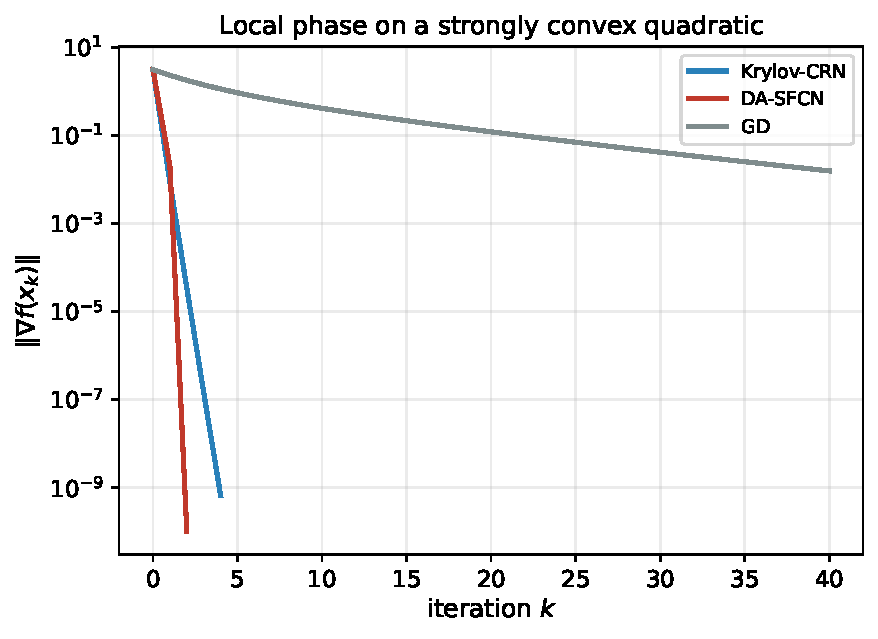
\includegraphics[width=0.49\textwidth]{fig_local.pdf}
\caption{يسار: الشهادة الطيفية على روزنبروك. يمين: الوعاء التربيعي المحلي.}
\end{figure}

\begin{table}[t]
\centering
\caption{إحصاءات ختامية مختارة.}
\small
\begin{tabular}{@{}llrrr@{}}
\toprule
المسألة & الطريقة & التكرارات & $\|g\|$ & \texttt{hvp} \\
\midrule
سرج $n=80$ & \textenglish{DA-SFCN} & 80 & $1.5\times10^{-7}$ & 1219 \\
سرج $n=80$ & \textenglish{LK-Newton} & 30 & $5.9\times10^{-12}$ & 158 \\
سرج $n=80$ & \textenglish{SFN} & 17 & $1.2\times10^{-9}$ & 204 \\
سرج $n=80$ & تدرّج & 80 & $4.2\times10^{-1}$ & 0 \\
لوجستي & \textenglish{DA-SFCN} & 6 & $4.8\times10^{-13}$ & -- \\
تحليل مصفوفات & \textenglish{DA-SFCN} & 19 & $9.8\times10^{-14}$ & -- \\
وعاء محلي & \textenglish{DA-SFCN} & 2 & $1.0\times10^{-10}$ & -- \\
وعاء محلي & تدرّج & 40 & $1.6\times10^{-2}$ & 0 \\
\bottomrule
\end{tabular}
\end{table}

\section{المناقشة والقيود}
ثلاثة دروس: (1) الفضاء الطيفي يهزم الإحداثي العشوائي؛ (2) الخلو من السرج
والتنظيم التكعيبي متكاملان لا بديلان؛ (3) $m_k$ الديناميكي محايد المعدل
موفِّر التكلفة. القيود: الأبعاد معتدلة ($n\le 80$)، ولم ندرج بعد الشبكات
العميقة ولا ضبط نماذج اللغة مقابل \textenglish{Sophia}/\textenglish{AdamW}.
والتحليل المحلّي للكسول والفيدرالي تحت انحراف العملاء ما يزال مفتوحًا.

\section{الخاتمة}
\textenglish{DA-SFCN} طريقة نيوتن تكعيبية واحدة، قابلة للتنفيذ، واعية
طيفيًا، خالية من السرج، متكيفة البعد، بمعدل عالمي $O(k^{-2/3})$ وضمان
تربيعي محلي تحت جدولة لوغاريتمية. والامتدادات الخمسة تُظهر أن النواة نفسها
تنتقل إلى الأوراكل العشوائي والجبر الكسول والإحماء من الرتبة الأولى
والبيانات الفيدرالية والقطع الموجَّه بالمتبقي. معًا تشكّل برنامج دكتوراه
متسقًا: فكرة واحدة، ست خوارزميات، نمط برهان مشترك، قاعدة شيفرة مشتركة،
وصورة تجريبية مشتركة.

\begin{english}
\begin{thebibliography}{20}
\bibitem{nesterov2006} Y.~Nesterov, B.~T.~Polyak. Cubic regularization of
Newton method. \textit{Math.\ Program.}, 2006.
\bibitem{cartis2011} C.~Cartis, N.~Gould, Ph.~Toint. Adaptive cubic
regularisation. \textit{Math.\ Program.}, 2011.
\bibitem{gower2019} R.~Gower et al. RSN. \textit{NeurIPS}, 2019.
\bibitem{hanzely2020} F.~Hanzely et al. SSCN. \textit{ICML}, 2020.
\bibitem{zhao2025} J.~Zhao, A.~Lucchi, N.~Doikov. SSCN-NC. \textit{AISTATS}, 2025.
\bibitem{jiang2024} R.~Jiang et al. Krylov CRN. \textit{AISTATS}, 2024.
\bibitem{dauphin2014} Y.~Dauphin et al. Saddle-free Newton. \textit{NeurIPS}, 2014.
\bibitem{oleary2020} T.~O'Leary-Roseberry et al. Low rank SFN. arXiv:2002.02881.
\bibitem{dembo1982} R.~Dembo, S.~Eisenstat, T.~Steihaug. Inexact Newton. \textit{SINUM}, 1982.
\bibitem{ge2016} R.~Ge, J.~Lee, T.~Ma. Matrix completion. \textit{NeurIPS}, 2016.
\bibitem{jin2017} C.~Jin et al. Escape saddle points. \textit{ICML}, 2017.
\bibitem{johnson2013} R.~Johnson, T.~Zhang. SVRG. \textit{NeurIPS}, 2013.
\bibitem{doikov2023} N.~Doikov et al. Lazy Hessians. \textit{ICML}, 2023.
\bibitem{mcmahan2017} H.~B.~McMahan et al. FedAvg. \textit{AISTATS}, 2017.
\bibitem{tripuraneni2018} N.~Tripuraneni et al. Stochastic cubic regularization. \textit{NeurIPS}, 2018.
\bibitem{pasechnyuk2025} D.~Pasechnyuk-Vilensky et al. VR cubic Newton. arXiv:2510.08714.
\bibitem{saad2003} Y.~Saad. Iterative Methods for Sparse Linear Systems. SIAM, 2003.
\bibitem{nocedal2006} J.~Nocedal, S.~Wright. Numerical Optimization. Springer, 2006.
\bibitem{liu2023} H.~Liu et al. Sophia. \textit{ICLR}, 2024.
\end{thebibliography}
\end{english}
\end{document}
